\documentclass{article}
\usepackage[utf8]{inputenc}
\usepackage{geometry}
\geometry{a4paper, margin=1.2in}
\usepackage{titling}
\usepackage{indentfirst}
\usepackage{biblatex}
\addbibresource{2023-01-24 References.bib}
\usepackage{graphicx}
\usepackage{url}

\title{\vspace{-2.0cm}Group Project Proposal}
\author{Group Orange}
\date{24 January 2023}

\begin{document}

\maketitle

\section{Introduction}
With great power comes great responsibility, and also great vigilance. The competition and bloodshed that accompanies being either a direct successor or on the throne itself is a well-known fact throughout existing monarchies around the world \cite{eisner-2011,kokkonen-2014}.
The desire and desperation to attain dominion over an entire kingdom  have pushed royalty to even poison, hang, stab, or even falsely accuse their siblings or parents of scandal \cite{saint-amand-1993}.
With such a bloodthirsty and dangerous  environment, it is likely that most royals did not survive until old age. 
However, different time periods ushers can cause varying influences on the extent of a royal’s lifespan. 
To explore this variation, this paper seeks to examine the question of \textbf{the lifespan of royals across the world through the centuries} and additional factors that might influence this. 
In order to investigate this research question, the longest, shortest, and average lifespans per century will be analyzed. 
Standard deviation will also be explored for individual centuries. 
To also evaluate the possible factors, the number of spouses and region of birth of royalty are considered against the lifespan. 

\section{Method}
The data set extracted was from the category The People of Wikipedia on DBpedia, a database that organizes Wikipedia pages and its data into syntax that can be utilized for analyses. This specific database  consists of various information about individuals, and was provided in a list of dictionaries .json format. It was first cleaned with Python through filtering dictionaries that contained ”royalty” label keys. Initially, we considered analyzing the relationship between lifespan against the number of heirs or children, and relatives. This data set however, did not contain a concrete definition for either categories or sufficient data. Relatives did not define the type of relative, and heirs were not present post-filtering.  Additionally, the only ‘heir’ data present pertained to the successor however this would not contribute to the research question. Furthermore, filtering by the label 'monarch' did not only give us royalties but also anyone who was related to that monarch. Therefore, we had to change both independent and dependent variables. Other necessary keys such as title, ontology/title, death place, birth place, number of spouses, and birth and death year were also included. Then, results were saved as a single .json file and converted into a .csv file. In the .csv file, we filtered the data into 3370 observations. Prior to specific data analysis,  a new column was created for lifespan calculated on the basis of birth year subtracted from death year.  An additional filter to ignore death years smaller than birth year was added to allow only positive age values. Then, we grouped years into different centuries to find the average lifespan of the royals to plot the data.

\section{Result}
Looking at the average lifespan of royals across centuries (figure 1), there is a trend of increasing the average life span throughout the centuries. Even though there are fluctuations before the 10th century. the general pattern we observe from this figure is an ascending pattern. 

From the impact of number of spouses on the lifespan of royalty (figure 2), we do not have clear trends to discuss because the number of spouses verses lifespan does not show any significant relationship. 

\begin{figure}[h!]
    \centering
    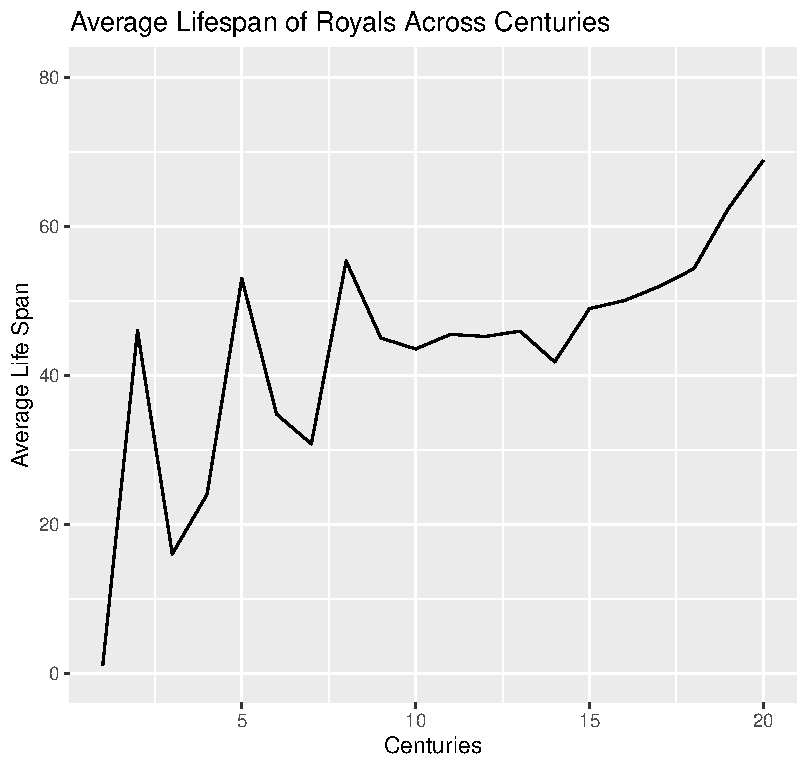
\includegraphics[width=10cm]{Average Lifespan of Royals Across Centuries.pdf}
    \caption{Average Lifespan of Royals Across Centuries}
    \label{fig:my_label}
\end{figure}

\begin{figure}[h!]
    \centering
    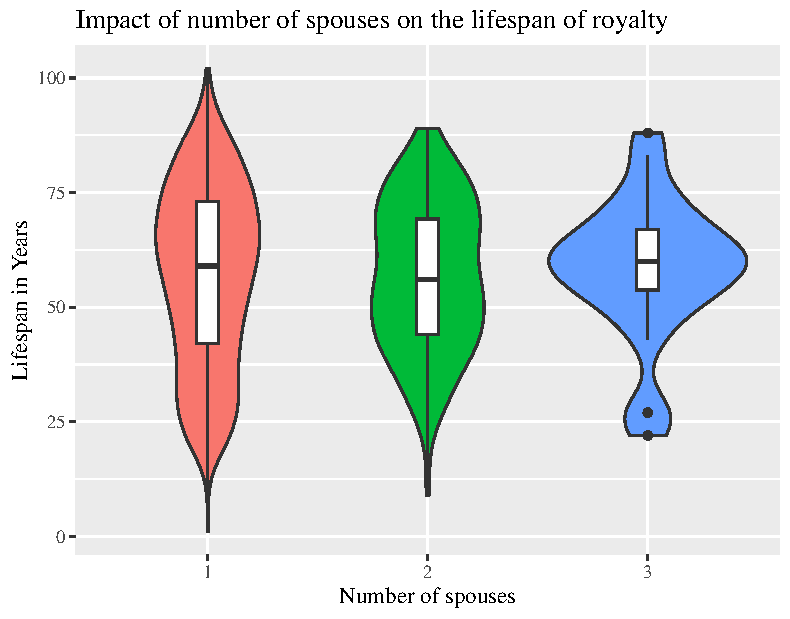
\includegraphics[width=10cm]{spouse_lifespan_violin.pdf}
    \caption{Average Lifespan of Royals based on the number of spouses}
    \label{fig:my_label}
\end{figure}

\section{Discussion}
Some of the limitations of this paper are that the number of royals in a century differs a lot from century to century. For example, the 1st century has only 1 royal who lived for a year, which would be considered an outlier. Also, during the data cleaning process, 7662 data points were removed if there were missing values, which could possibly have removed the majority of the royals from the earlier centuries due to a lack of records. 

\printbibliography

\section{Appendix}
\subsection{Data Questions}

\begin{enumerate}
    \item In which century did royalty have the longest lifespan? 
    \item In which century did royalty have the shortest lifespan? 
    \item What is the average lifespan in each century (time period)? (line graph) 
    \item (to do) What is the standard deviation  in each century? 
    \item (to do) Does the number of spouses affect the lifespan of a royal? 
    \begin{enumerate}
        \item A violin plot looking at variation in lifespan depending on 1-3 spouses
    \end{enumerate}
    \item (to do) Do some regions’ royalty have a longer lifespan than others? 
\end{enumerate}

\end{document}

\print